% !TEX TS-program = pdflatex
% !TEX encoding = UTF-8 Unicode

% This is a simple template for a LaTeX document using the "article" class.
% See "book", "report", "letter" for other types of document.

\documentclass[11pt]{article} % use larger type; default would be 10pt

\usepackage[utf8]{inputenc} % set input encoding (not needed with XeLaTeX)

%%% Examples of Article customizations
% These packages are optional, depending whether you want the features they provide.
% See the LaTeX Companion or other references for full information.

%%% PAGE DIMENSIONS
\usepackage{geometry} % to change the page dimensions
\geometry{letterpaper} % or letterpaper (US) or a5paper or....
% \geometry{margin=2in} % for example, change the margins to 2 inches all round
% \geometry{landscape} % set up the page for landscape
%   read geometry.pdf for detailed page layout information

\usepackage{graphicx} % support the \includegraphics command and options

% \usepackage[parfill]{parskip} % Activate to begin paragraphs with an empty line rather than an indent

%%% PACKAGES
\usepackage{booktabs} % for much better looking tables
\usepackage{array} % for better arrays (eg matrices) in maths
\usepackage{paralist} % very flexible & customisable lists (eg. enumerate/itemize, etc.)
\usepackage{verbatim} % adds environment for commenting out blocks of text & for better verbatim
\usepackage{subfig} % make it possible to include more than one captioned figure/table in a single float
% These packages are all incorporated in the memoir class to one degree or another...

%%% HEADERS & FOOTERS
\usepackage{fancyhdr} % This should be set AFTER setting up the page geometry
\pagestyle{fancy} % options: empty , plain , fancy
\renewcommand{\headrulewidth}{0pt} % customise the layout...
\lhead{}\chead{}\rhead{}
\lfoot{}\cfoot{\thepage}\rfoot{}

%%% SECTION TITLE APPEARANCE
\usepackage{sectsty}
\allsectionsfont{\sffamily\mdseries\upshape} % (See the fntguide.pdf for font help)
% (This matches ConTeXt defaults)

%%% ToC (table of contents) APPEARANCE
\usepackage[nottoc,notlof,notlot]{tocbibind} % Put the bibliography in the ToC
\usepackage[titles,subfigure]{tocloft} % Alter the style of the Table of Contents
\renewcommand{\cftsecfont}{\rmfamily\mdseries\upshape}
\renewcommand{\cftsecpagefont}{\rmfamily\mdseries\upshape} % No bold!

%%% END Article customizations

\renewcommand\thesubsection{\alph{subsection})}

%%% The "real" document content comes below...
\usepackage[normalem]{ulem}

\title{Assignment 6: Rayleigh Quotient Iteration; Splitting Methods}
\author{ Gregory \uline{Smetana} \\ID 1917370 \\ ACM 106a }
%\date{} % Activate to display a given date or no date (if empty),
         % otherwise the current date is printed 

\usepackage{fancyhdr}
\usepackage{lastpage}

\usepackage{../mcode}

\usepackage{mathtools}
\pagestyle{fancy}
\lhead{Gregory \uline{Smetana}}
\rhead{ID 1917370 }


\begin{document}


\maketitle


\section{The spectral radius}
The spectral radius of the matrix $A$ is defined as
\begin{equation}
\rho(A) = \max \{| \lambda | : \lambda \mbox{ is an eigenvalue of } A \}
\label{eq:spectral}
\end{equation}

\subsection{} %1a
\begin{equation}
\begin{split}
\| A \|_2 &= \substack{\max \\ \|x\|\ne 0} \frac{\|A x \|_2}{\|x\|_2}\\
&=  \substack{\max \\ \|x\|\ne 0} \frac{\sqrt{x^* A^* A x}}{\|x\|_2}
\end{split}
\end{equation}
The matrix $A^*A$ is Hermitian, so there exists an eigendecomposition $A^* A = Q D Q^*$ with $D = $ diag$(\lambda_1, ... , \lambda_n)$, where $\lambda_1 \ge \lambda_2 \ge ... \ge \lambda_n \ge 0$. 
\begin{equation}
\begin{split}
\| A \|_2 &=\substack{\max \\ \|x\|\ne 0} \frac{\sqrt{x^* Q D Q^* x}}{\|x\|_2}\\
&=\substack{\max \\ \|x\|\ne 0} \frac { \sqrt{x^* Q D Q^* x}}{\|x\|_2}\\
&=\substack{\max \\ \|x\|\ne 0} \frac { \sqrt{(Q^*x)^* D Q^* x}}{ \|Qx\|_2}\\
&=\substack{\max \\ \|y\|\ne 0} \frac { \sqrt{y^* D y}}{ \|y\|_2}\\
&=\substack{\max \\ \|y\|\ne 0} \sqrt{ \frac{\sum \lambda_i y_i^2}{\sum y_i^2}}\\
&= \sqrt{\lambda_1(A^*A)} = \sigma_1(A)
\end{split}
\end{equation}
Thus we have shown that $ \| A \|_2 = \sigma_1(A)$. From the last line above, it was shown that
\begin{equation}
\|A \|_2 = \sqrt{ \rho(A^* A)}
\end{equation}
For the special case of $A$ symmetric, the eigenvalues of $A^*A = A^2 =Q D^2 Q^*$ are the squares of the eigenvalues of $A$, so
\begin{equation}
\|A \|_2 = \sqrt{ \rho(A^* A)} = \sqrt{ \rho(A)^2} =\rho(A)
\end{equation}
Therefore,
\begin{equation}
\boxed{\rho(A)=\sigma_1(A) = \|A \|_2 }
\end{equation}
\subsection{} %1b
The statement  $\|A \|_2 = \rho(A)$ is false for a general matrix $A$. In particular, we examine the matrix
\begin{equation}
A = \left ( \begin{array}{rr}
1 &m \\
0 & 1 \\
\end{array} \right )
\end{equation}
\begin{equation}
0=\det \left ( \begin{array}{rr}
1-\lambda &m \\
0 & 1-\lambda \\
\end{array} \right ) = (1-\lambda)^2
\end{equation}
so we have $\rho(A)  =1$
\begin{equation}
\| A \|_2 = \substack{\max \\ \|x =1\|} \|A x \|_2
\end{equation}
\begin{equation}
\| A \|_2 \ge \| \left ( \begin{array}{rr}
1 &m \\
0 & 1 \\
\end{array} \right )\left ( \begin{array}{r}
0 \\
1\\
\end{array} \right )\|_2 = \| \left ( \begin{array}{r}
m \\
1\\
\end{array} \right )\|_2 = \sqrt{1+m^2}
\end{equation}
Therefore $A$ satisfies $\| A\|_2 > m$ and $\rho(A) < \|A\|_2$ if $m\ge1$.
%\begin{equation}
%A^*A  = \left ( \begin{array}{rr}
%1 &m \\
%m & 1+m^2 \\
%\end{array} \right )
%\end{equation}
%\begin{equation}
%0=\det \left ( \begin{array}{rr}
%1-\lambda &m \\
%m & 1+m^2-\lambda \\
%\end{array} \right ) = (1-\lambda)( 1+m^2-\lambda ) -m^2
%\end{equation}
%\begin{equation}
%\lambda = \frac{1}{2}\left (2+m^2 \pm m\sqrt{4+m^2} \right )
%\end{equation}
%\begin{equation}
%\sigma_1 = \sqrt{ \frac{1}{2}\left (2+m^2 + m\sqrt{4+m^2} \right ) } > m
%\end{equation}
%Therefore,
%\begin{equation}
%\| A \|_2 > m
%\end{equation}
We have shown that we may have $\rho(A) < \| A \|_2$ if $A$ is not Hermitian.
\subsection{} %1c
\begin{equation}
A x = \lambda x
\end{equation}
Multiplying by $A$ on both sides and substituting $A = \lambda x$ on the right, we have
\begin{equation}
A^r x =\lambda^r x
\end{equation}
\begin{equation}
\| A^r x \| = | \lambda^r | \|x\|
\end{equation}
for an operator norm, $ \| A^r x \| \le \|A^r \| \|x\|$, so
\begin{equation}
\|A^r \| \|x\| \ge | \lambda^r | \|x\|
\end{equation}
\begin{equation}
\|A^r \| \ge | \lambda^r |
\end{equation}
therefore
\begin{equation}
\boxed{\rho(A) \le \|A^r \|^{1/r}}
\end{equation}
for any operator norm $\| \cdot \|$ and positive $r$
\subsection{} %1d
A normal matrix is diagonalizable. Therefore, we may express
\begin{equation}
A = Q D Q^* = \sum_i^n \lambda_i q_i q_i^*
\end{equation}
with $D = $ diag$(\lambda_1, ... , \lambda_n)$, $\lambda_i \in \mathbf{R}$ and eigenvectors $q_i$ normalized such that $\|q_i\| = 1$
\begin{equation}
A^r  = \sum_{i=1}^n \lambda_i^r q_i q_i^*
\end{equation}
Now consider the norm of $A^r$ divided by the spectral radius with $r \rightarrow \infty$
\begin{equation}
\lim_{r \rightarrow \infty} \frac{\| A^r \|}{\rho(A)^r}=\lim_{r \rightarrow \infty} \| \sum_{i=1}^n \frac{\lambda_i^r q_i q_i^*}{\rho(A)^r} \|
\end{equation}
 The terms may be grouped by unique magnitude of eigenvalue. Say that  there are $m \le n$ unique magnitudes  $|\lambda_i|$ with  $k_i$ associated terms in the sum. Using norm inequalities and Equation~\ref{eq:spectral} to write $\rho(A) = | \lambda_{max} |$, we may rewrite the sum:
\begin{equation}
\lim_{r \rightarrow \infty} \frac{\| A^r \|}{\rho(A)^r} \le \lim_{r \rightarrow \infty}  \sum_{i=1}^m \frac{| \lambda_i^r | }{| \lambda_{max}^r |} \|\sum_{j=1}^{k_i} q_{i,j} q_{i,j}^* \| 
\end{equation}
Now we will show that
\begin{equation}
\| \sum_{j=1}^{k} q_{j} q_{j}^* \| =1
\end{equation}
Starting with the definition of the norm
\begin{equation}
 \|  \sum_{j=1}^{k} q_j q_j^* \| = \substack{\max \\ \|x\|=1} \| \sum_{j=1}^{k} q_j q_j^* x \|
\end{equation} 
Expressing $x$ in the basis of $n$ eigenvectors, $x = \sum_{i=1}^n \alpha_i q_i $
\begin{equation}
\|  \sum_{j=1}^{k} q_j q_j^* \| = \substack{\max \\ \|x\|=1} \| \sum_{j=1}^{k} \alpha_j q_j \|
\end{equation}
\begin{equation}
\| \sum_{j=1}^{k} \alpha_j q_j \| \le \| \sum_{i=1}^n \alpha_i q_i \| = \| x \| = 1
\end{equation}
so it is maximized when $x$ is written in the basis of $k$ eigenvectors, $x =  \sum_{j=1}^{k} \alpha_j q_j$. We see that 
\begin{equation}
\| \sum_{j=1}^{k} q_{j} q_{j}^* \| =1
\end{equation}
Therefore,
\begin{equation}
\lim_{r \rightarrow \infty} \frac{\| A^r \|}{ \rho(A)^r} \le \lim_{r \rightarrow \infty}  \sum_{i=1}^m \frac{| \lambda_i^r | }{| \lambda_{max}^r |}
\end{equation}
As $r \rightarrow \infty$, only the term corresponding to the maximum eigenvalue magnitude will not vanish, so
\begin{equation}
\lim_{r \rightarrow \infty} \frac{\| A^r \|}{ \rho(A)^r} \le 1
\end{equation}
Combined with the previous result which stated
\begin{equation}
 \frac{\| A^r \|}{ \rho(A)^r} \ge 1
\end{equation}
we have shown that
\begin{equation}
\frac{A^r}{\rho(A)^r} \rightarrow 1
\end{equation}
Therefore
\begin{equation}
\boxed{\rho(A) = \lim_{r \rightarrow \infty} \|A^r \|^{1/r} }
\end{equation}
\section{Convergence of the Jacobi and Gauss-Seidel methods}
A splitting method converges if and only if the update matrix $R$ has spectral radius satisfying
\begin{equation}
 \rho(R) < 1 
\end{equation}
The update matrix of the Jacobi method is 
\begin{equation}
R_J = L + U
\end{equation}
The update matrix of Gauss-Seidel is
\begin{equation}
R_{GS} = (I-L)^{-1} U
\end{equation}
where we adopt the Demmel notation of 
\begin{equation}
A = D - \tilde{L} - \tilde{U} = D(I - L - U )
\end{equation}
where $-\tilde{L} = - D L $ is the strictly lower triangular part of $A$ and $-\tilde{U} = -UL$ is the strictly upper triangular part of $A$.
\subsection{} %2a
Suppose $A x = b$, where $A \in \mathbf{R}^{2 \times 2}$ is symmetric positive definite. This means $A$ is symmetric and $x^T A x > 0$ for all $x \in \mathbf{R}^2$, or equivalently, all eigenvalues of $A$ are positive.

Consider
\begin{equation}
A = \left ( \begin{array}{rr}
a &b \\
b & c \\
\end{array} \right )
\end{equation}

The eigenvalues of $A$ are found with the characteristic polynomial:
\begin{equation}
	0 = (a- \lambda)(c-\lambda) - b^2
\end{equation}
\begin{equation}
\lambda = \frac{1}{2} \left ( a + c \pm \sqrt{a^2 +4b^2 - 2ac +c^2}\right )
\end{equation}
The eigenvalues must be positive, so we see the trace and determinant must be positive:
\begin{equation}
a +c > 0
\end{equation}
\begin{equation}
ac -b^2  > 0
\end{equation}
For this matrix, we have
\begin{equation}
L =  \left ( \begin{array}{rr}
0 &0 \\
-b/c & 0 \\
\end{array} \right )
\end{equation}
\begin{equation}
U =  \left ( \begin{array}{rr}
0 &-b/a\\
0 & 0 \\
\end{array} \right )
\end{equation}
\begin{equation}
R_J= L +U  = \left ( \begin{array}{rr}
0 &-b/a \\
-b/c & 0 \\
\end{array} \right )
\end{equation}
Solving for the eigenvalues of $R_J$,
\begin{equation}
\lambda_J^2 -\frac{ b^2}{ac} = 0
\end{equation}
\begin{equation}
\lambda_J = \pm \frac{b}{\sqrt{ac}}
\end{equation}
The spectral radius shows that the Jacobi method converges for the matrix $A$:
\begin{equation}
\boxed{\rho(R_J) = b^2/ac < 1}
\end{equation}
Using the identity of the inverse of a $2 \times 2$ matrix to find $R_{GS}$,
\begin{equation}
\begin{split}
R_{GS}& =(I-L)^{-1} U \\
& = \left ( \begin{array}{rr}
1 &0 \\
b/c & 1 \\
\end{array} \right )^{-1}
\left ( \begin{array}{rr}
0 & -b/a \\
0 & 0 \\
\end{array} \right )\\
&= \left ( \begin{array}{rr}
1 &0\\
-b/c & 1 \\
\end{array} \right )
\left ( \begin{array}{rr}
0 & -b/a \\
0 & 0 \\
\end{array} \right )\\
&=\left ( \begin{array}{rr}
0 & -b/a \\
0 & b^2/ac \\
\end{array} \right )
\end{split}
\end{equation}
Solving for the eigenvalues of $R_{GS}$,
\begin{equation}
\lambda_{GS} = \{0, b^2/ac \}
\end{equation}
The spectral radius shows that the Gauss-Seidel method converges:
\begin{equation}
\boxed{\rho(R_{GS}) = b^2/ac < 1}
\end{equation}
\subsection{} %2b
Now consider the $2 \times 2$ matrix
\begin{equation}
A = \left ( \begin{array}{rr}
1 & \alpha \\
-\alpha & 1 \\
\end{array} \right )
\end{equation}
For this matrix,
\begin{equation}
L =  \left ( \begin{array}{rr}
0 &0 \\
\alpha & 0 \\
\end{array} \right )
\end{equation}
\begin{equation}
U =  \left ( \begin{array}{rr}
0 & -\alpha\\
0 & 0 \\
\end{array} \right )
\end{equation}
\begin{equation}
R_J= L +U  = \left ( \begin{array}{rr}
0 & -\alpha \\
\alpha & 0 \\
\end{array} \right )
\end{equation}
Computing the eigenvalues of $R_J$,
\begin{equation}
\lambda_J =\pm i \alpha
\end{equation}
The spectral radius shows that the Jacobi method converges when
\begin{equation}
\boxed{\rho(R_J) =|  \alpha |< 1}
\end{equation}
\begin{equation}
\begin{split}
R_{GS}& =(I-L) ^{-1} U \\
&= \left ( \begin{array}{rr}
1 &0 \\
-\alpha & 1 \\
\end{array} \right )^{-1}
\left ( \begin{array}{rr}
0 & -\alpha \\
0 & 0 \\
\end{array} \right )\\
&= \left ( \begin{array}{rr}
1 &0 \\
\alpha & 1 \\
\end{array} \right )
\left ( \begin{array}{rr}
0 & -\alpha \\
0 & 0 \\
\end{array} \right )\\
&=\left ( \begin{array}{rr}
0 & -\alpha \\
0 & -\alpha^2 \\
\end{array} \right )
\end{split}
\end{equation}
Computing the eigenvalues of $R_{GS}$,
\begin{equation}
\lambda_{GS} = \{ 0, -\alpha^2 \}
\end{equation}
The spectral radius shows that the Gauss-Seidel method converges when
\begin{equation}
\boxed{\rho(R_{GS}) =| \alpha^2| < 1}
\end{equation}
\subsection{} %2c
 Now consider the $2 \times 2$ block matrix
\begin{equation}
A = \left ( \begin{array}{rr}
I & S \\
-S^T & I \\
\end{array} \right )
\end{equation}
For this matrix,
\begin{equation}
L =  \left ( \begin{array}{rr}
0 &0 \\
S^T & 0 \\
\end{array} \right )
\end{equation}
\begin{equation}
U =  \left ( \begin{array}{rr}
0 & -S\\
0 & 0 \\
\end{array} \right )
\end{equation}
\begin{equation}
R_J= L +U  = \left ( \begin{array}{rr}
0 & -S \\
S^T & 0 \\
\end{array} \right )
\end{equation}
Computing the eigenvalues of $R_J$,
\begin{equation}
\det \left ( \begin{array}{rr}
-\lambda_J I & -S \\
S^T & -\lambda_J I \\
\end{array} \right )=0
\end{equation}
We may use an identity for the determinant of a block matrix:
\begin{equation}
\det \left ( \begin{array}{rr}
A & B \\
C & D \\
\end{array} \right ) = \det(AD - BC)
\end{equation}
where the blocks are square matrices and $C$ and $D$ commute ($CD = DC$)
\begin{equation}
0= \det(\lambda_J^2 I + S S^T) 
\end{equation}
Using the singular value decomposition of  $S$,
\begin{equation}
S = U \Sigma V^T
\end{equation}
where
\begin{itemize}
\item $U \in \mathbf{R}^{n\times n}$ such that $U^T U = I$
\item $V \in \mathbf{R}^{n\times n}$ such that $V^T V = I$
\item $\Sigma =$ Diag$(\sigma_1, \sigma_2, ... , \sigma_n)$ where $\sigma_1 \ge \sigma_2 \ge ... \ge \sigma_n \ge 0$. 
\end{itemize}
we have
\begin{equation}
\begin{split}
0&= \det(\lambda_J^2 I + U \Sigma^2 U^T) \\
&= \det(U( \lambda_J^2 I + \Sigma^2 )U^T) \\
& = \det(U) \det(\lambda_J^2 I + \Sigma^2) \det(U^T)
\end{split}
\end{equation}
The determinant of a unitary matrix is $\pm 1$, so we must have
\begin{equation}
0=\det(\lambda_J^2 I + \Sigma^2) = \det \left ( \begin{array}{rrr}
\lambda_J^2 + \sigma_1^2 &&0 \\
& \ddots & \\
0&& \lambda_J^2 + \sigma_n^2 \\
\end{array} \right )
\end{equation}
with
\begin{equation}
\lambda_{J,i} = \pm i \sigma_i
\end{equation}
The spectral radius shows that the Jacobi method converges when
\begin{equation}
\boxed{\rho(R_{J}) =\sigma_1 < 1}
\end{equation}
Now examining the Gauss-Seidel algorithm,
\begin{equation}
\begin{split}
R_{GS}&=(I-L)^{-1} U \\
&= \left ( \begin{array}{rr}
I  &0 \\
-S^T & I \\
\end{array} \right )^{-1}
\left ( \begin{array}{rr}
0 & -S \\
0 & 0 \\
\end{array} \right )
\end{split}
\end{equation}
Using the blockwise inversion formula
\begin{equation}
\left ( \begin{array}{rr}
A & B \\
C & D \\
\end{array} \right ) ^{-1}= 
\left ( \begin{array}{rr}
A^{-1}+A^{-1}B(D-CA^{-1}B)^{-1}CA^{-1} & -A^{-1}B(D-CA^{-1}B)^{-1} \\
-(D-CA^{-1}B)^{-1}CA^{-1}&(D-CA ^{-1}B)^{-1}\\
\end{array} \right ) 
\end{equation}
with $B=0$, $C=-S^T$, and $A=D=I$, we have
\begin{equation}
\begin{split}
R_{GS} &=\left ( \begin{array}{rr}
I  & 0 \\
S^T & I \\
\end{array} \right ) 
\left ( \begin{array}{rr}
0 & -S \\
0 & 0 \\
\end{array} \right ) \\
& = \left ( \begin{array}{rr}
0 & -S \\
0 & -S^T S \\
\end{array} \right )
\end{split}
\end{equation}
Computing the eigenvalues of $R_{GS}$,
\begin{equation}
\begin{split}
0&=\det\left ( \begin{array}{rr}
-\lambda_{GS}I & -S \\
0 & -S^T S- \lambda_{GS} I \\
\end{array} \right ) \\
& =\det \left ( \lambda_{GS} S^T S +  \lambda_{GS}^2 I  \right )
\end{split}
\end{equation}
Using the singular value decomposition $S = U \Sigma V^T$,
\begin{equation}
\begin{split}
0&= \det \left( \lambda_{GS} V \Sigma^2 V^T + \lambda_{GS}^2 I \right ) \\
& = \det \left ( V \left ( \lambda_{GS} \Sigma^2 + \lambda_{GS}^2 I \right ) V^T \right ) \\
& = \det (V) \det \left ( \lambda_{GS} \Sigma^2 + \lambda_{GS}^2 I \right ) \det(V^T)
\end{split}
\end{equation}
Since the determinant of a unitary matrix is $\pm 1$, we must have
\begin{equation}
0=\det \left ( \lambda_{GS} \Sigma^2 + \lambda_{GS}^2 I \right )  = \det \left ( \begin{array}{rrr}
\lambda_{GS} (\lambda_{GS} + \sigma_1^2)  &&0 \\
& \ddots & \\
0&& \lambda_{GS} (\lambda_{GS} + \sigma_n^2) \\
\end{array} \right )
\end{equation}
so we have
\begin{equation}
\lambda_{GS} = \{ 0, -\sigma_i^2\}
\end{equation}
The spectral radius shows that the Gauss-Seidel method converges when
\begin{equation}
\boxed{\rho(R_{GS}) =\sigma_1^2 < 1}
\end{equation}
\section{Rayleigh Quotient Iteration}
\subsection{} %3a
Rayleigh Quotient iteration as described in Demmel Algorithm 5.1 was implemented in Matlab in \verb$rayleigh_quotient.m$. The ``$\backslash$" solver was used to solve linear systems.
\subsection{} %3b
A random $4\times4$ orthogonal matrix $U$ was used to generate
\begin{equation}
A = U DU^T
\end{equation}
where $D =$ Diag($2, 4, 13, 27)$.  The starting point for each Rayleigh Quotient iteration was chosen as 10 times the one column of $U$ plus a random combination of the other columns. This led to convergence of each eigenvector of $A$, which was verified by examination of the Rayleigh Quotients.

The error was measured as the forward error between the current Rayleigh quotient and desired eigenvalue. The error on a log scale as a function of the number of iterations is displayed in Figure~\ref{fig:p3b}.
\begin{figure}[h!]
  \centering
    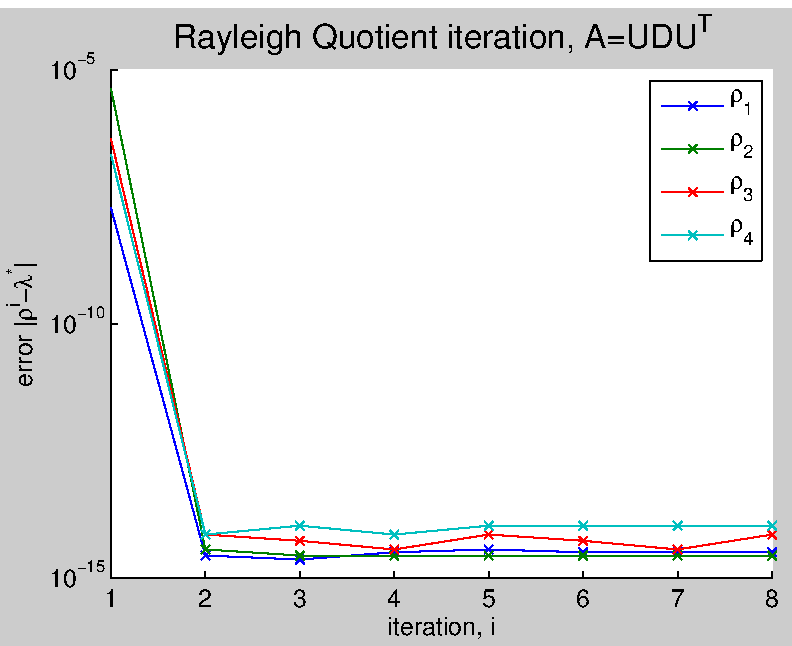
\includegraphics[width=0.7\textwidth]{p3b}
  \caption{}
\label{fig:p3b}
\end{figure}

The error at each step of the algorithm behaves like
\begin{equation}
e = c^{-r^k}
\end{equation}
where $c$ is some constant and $r$ is the rate of convergence. 
so we have
\begin{equation}
\log(\log(e)) = \log(\log(c^{-r^k})) = \log(-r^k \log(c)) = k \log(-r )+ \log(\log (c))
\end{equation}

\begin{figure}[h!]
  \centering
    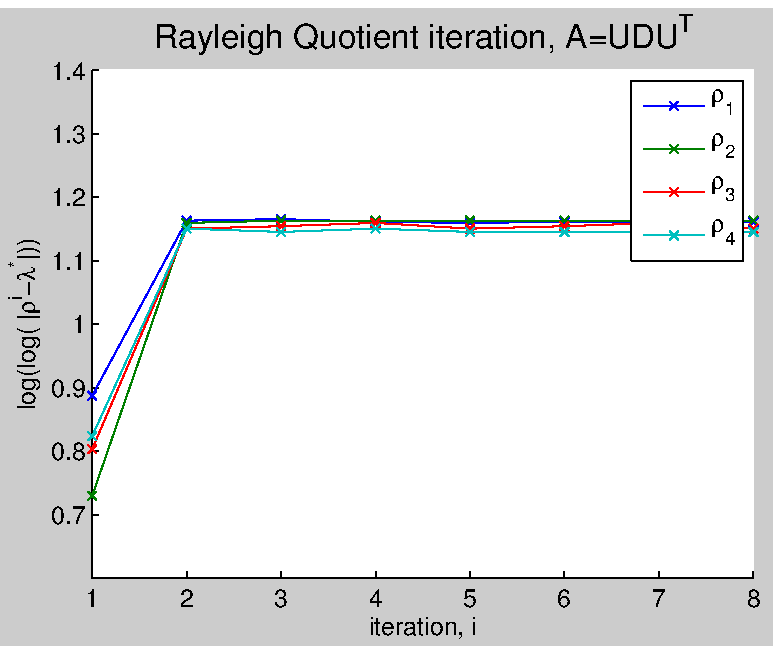
\includegraphics[width=0.7\textwidth]{p3blog}
  \caption{}
\label{fig:p3blog}
\end{figure}
From the log-log plot in Figure~\ref{fig:p3blog}, we see that $\log(r) \sim 0.4$. Therefore the Rayleigh Quotient iteration converges roughly at a rate $r = 2.5$.
\subsection{} %3c
A random $4 \times 4$ matrix $S$ with $\kappa(S) =\sigma_1(S)/\sigma_4(S)=10$ was generated by taking the product of its singular value decomposition. Then Rayleigh Quotient iteration was performed on
\begin{equation}
A=SDS^{-1}
\end{equation}
The error on a log scale as a function of the number of iterations is displayed in Figure~\ref{fig:p3c}. From the log-log plot in Figure~\ref{fig:p3clog}, we see that $\log(r) \sim 0.25$, and the Rayleigh Quotient iteration converges roughly at a rate $r = 1.8$.
\begin{figure}[h!]
  \centering
    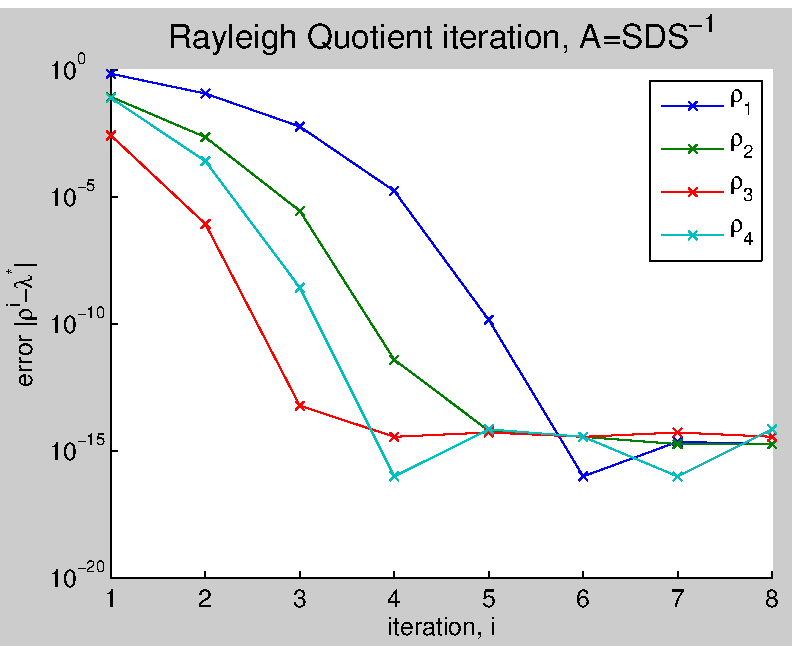
\includegraphics[width=0.7\textwidth]{p3c}
  \caption{}
\label{fig:p3c}
\end{figure}

\begin{figure}[h!]
  \centering
    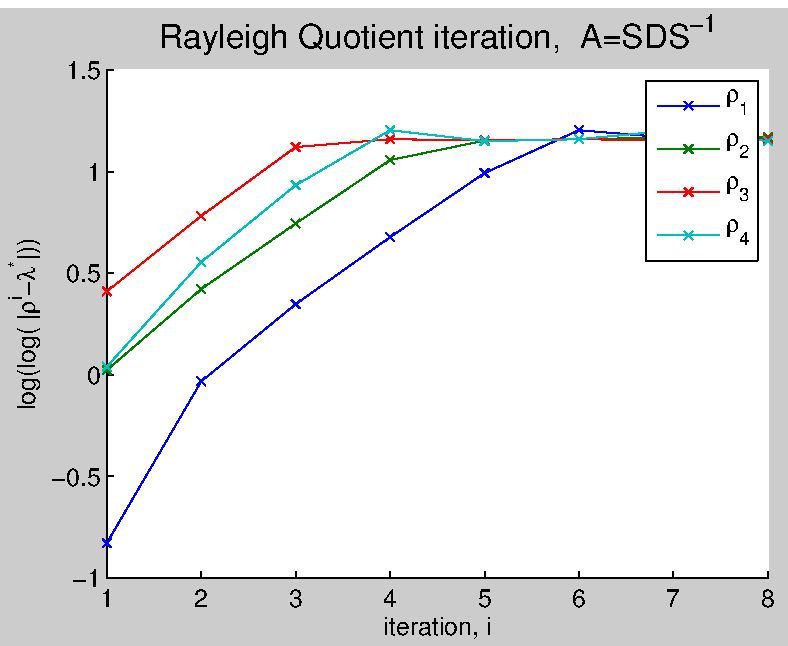
\includegraphics[width=0.7\textwidth]{p3clog}
  \caption{}
\label{fig:p3clog}
\end{figure}

\clearpage
\appendix
\section{rayleigh\_quotient.m}
\lstinputlisting{../rayleigh_quotient.m}
\section{Smetana\_Gregory\_1917370\_A6\_P3\_DIARY.txt}
\lstinputlisting{../Smetana_Gregory_1917370_A6_P3_DIARY.txt}

\section{Smetana\_Gregory\_1917370\_A6\_P3m}
\lstinputlisting{../Smetana_Gregory_1917370_A6_P3.m}

\end{document}

